\documentclass[12pt]{article}
\usepackage{mandi}
\usepackage{braket}
\usepackage{graphicsx}
\usepackage{amsmath}
\usepackage{amsfonts}
\usepackage{tikz}
\usepackage{epstopdf}
\tolerance=1
\emergencystretch=\maxdimen
\hyphenpenalty=10000
\hbadness=10000
% Palatino font (ppl must be installed).
\renewcommand*\rmdefault{ppl}
% Iwona font (iwona must be installed).
%\renewcommand*\rmdefault{iwona}
\begin{document}
\title{Implementation of Quantum Computing Techniques on NMR systems}
\author{Anurag Pallaprolu \\ 2012B5A3405P \\ BITS Pilani }
\maketitle
\begin{abstract}
This document is submitted as a partial requirement for the course Quantum Information and Computing, BITS Pilani. The phenomenon of NMR can be used to generate spin states of nuclei and these can be used as qubits for computational purposes, the speciality being, an ensemble of molecules must be utilized. According to ~\cite{JAJ}, it is both the best, and the worst technologies in quantum computing, reasons being the ease at which unitary quantum gates can be implemented and the difficulty in exact measurements without disturbing the ensemble respectively. 
\end{abstract}
\section{Introduction and NMR Terminologies}
\textbf{Nuclear Magnetic Resonance} is an important phenomenon in Physics, Chemistry and Medicine, was first discovered by \textbf{Isaac Isidor Rabi} in 1938, for which he won the Nobel Prize in 1944. Later, \textbf{Edward Mills Purcell} and \textbf{Felix Bloch} won the 1952 Nobel Prize \textit{for their developments of new methods for nuclear magnetic precision measurements and discoveries in connection therewith}.~\cite{npb}. The phenomenon occurs to certain nuclei, when placed in a strong static magnetic field, and are exposed to an oscillating magnetic field, depending on whether the nuclei possess intrinsic nucleonic spin or not. The concept of spin is quite simple as explained in the accompanying document ~\cite{me} and a fact that must be kept in mind is that we are talking about quantum mechanical version of spin and hence, we would be looking at things like Zeeman Effect etc,. When placed in a magnetic field of frequency $\mathbb{B}$, a particle with some net non-zero spin can absorb a photon of frequency $\nu$. The relationship being $$\nu = \gamma\mathbb{B}$$ The number $\gamma$ is called as the \textbf{gyromagnetic ratio} and depends on the particle at hand ~\cite{jph}. Simply seen, when any particle with a non zero spin is placed in a static magnetic field, it can stay in two energy levels, the lower energy level due to the straight pairing of N-S poles of the field to that of the particle, and the higher \textit{unstable} energy state of the anti-pairing of the N-S poles of the field with the particle.
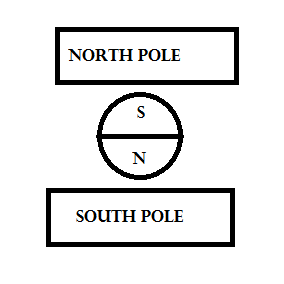
\includegraphics[scale=0.9]{nsns.png}
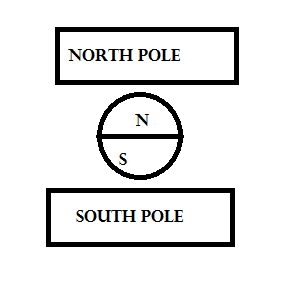
\includegraphics[scale=0.9]{nnss.png}

As we have seen, any transition from these two energy levels must be facilitated by quanta, according to Planck's hypothesis. Hence, we get the relation
$$E = h\gamma\mathbb{B}$$
When there is a lower level transition, or a photon arrives with the frequency equal to the \textbf{Larmor Frequency} given before, then a shift in the energy level happens~\cite{acadml}. In the case of \textbf{nuclear} magnetic resonance, the emission of photons or the absorbed photon usually lie in the radio frequency ranges of the electromagnetic spectrum. In NMR spectroscopy, $\nu$ is between 60 and 800 MHz for hydrogen nuclei. In clinical MRI, $\nu$ is typically between 15 and 80 MHz for hydrogen imaging ~\cite{jph}. The simplest possible implementation of NMR in actual atoms is the \textbf{Continuous Wave} NMR experiment. In this, you can either hold the magnetic field constant and supply RF pulses with varying frequency to note the absorbed energy, or, you can hold the pulsing frequency constant and vary the magnetic field to look for some resonance. The diagrams below should be helpful in making this point clear.

\begin{figure}
\begin{tikzpicture}[overlay]
\draw [<->,thick] (0,5) node (yaxis) [below] {Absorbed Energy}
        |- (5,0) node (xaxis) [right] {Frequency};
\draw [ultra thick, red] (0,0) -- (3,0)--(4,3)--(5,0)--(6,0);        
\end{tikzpicture}
\caption{The Energy-Frequency Diagram}
\end{figure}
\begin{figure}
\begin{tikzpicture}
\draw [<->,thick] (0,5) node (yaxis) [above] {Energy}
        |- (5,0) node (xaxis) [right] {Magnetic Field};

\draw (0,2.5) -- (4,4) --(6,4);
\draw (0,2.5) -- (4,1.5) --(6,1.5);
\draw [ultra thick, red] (3,1) -- (3,4);
\node [above] at (6,4) {Unpaired High Energy};
\node [above] at (6,1.5) {Paired High Energy};
\end{tikzpicture}
\caption{CWNMR Frequency Variation}
\end{figure}
\subsection{Ensemble}
Now, we shall move on to statistics of the spin particle ensembles. The problem with NMR spectroscopy is that the radio frequency photons are hard to detect, identify and measure as each one of them carries an energy of around $1\mu eV$. This leads to the following idea that, inorder to measure significant readings, an \textbf{ensemble} is required to be used experimentally. The number of molecules is approximated to be of the order of $10^{19}$ according to ~\cite{JAJ}. To analyze such large systems, we must comply to look at the \textit{macroscopic} point of view rather than the \textit{microscopic} one, and hence, we shall look at a bit of \textbf{Boltzmann statistics}. It is based on the probabilistic law that \textbf{Ludwig Boltzmann} proposed, and is very well explained in the standard ~\cite{Feyn}. We define $$\beta = \frac{1}{kT}$$ and then we can state from Boltzmann's law, that, 
$$\frac{N^{+}}{N^{-}} = e^{-\beta E}$$ where $N^+$ and $N^-$ are the number of particles in spin up and down states respectively and E is the energy difference between the two states. 
\begin{figure}
\begin{center}
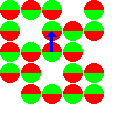
\includegraphics[scale=1]{ens1.png}
\end{center}
\caption{The Spin Packet of an Ensemble and the net $\mathbb{M}$ vector}
\end{figure}
Then, we take an ensemble and compartmentalize it into smaller boxes and call these \textbf{spin packets}. This then leads to the formulation of a magnetization vector $\mathbb{M}$ for each of these packets and it is obvious that $$\mathbb{M} =  \lambda (N^+ - N^-)$$ A system of axes can be set up here, with the z axis in the direction of $\mathbb{M}$. Let us take a deviation here, and look at the contributing Hamiltonian to NMR processes. According to the excellent paper ~\cite{ohio}, any atomic hamiltonian contains \textbf{nine important} terms that relate to any type of a quantum process. Let us look at them one by one. The first one is called the \textbf{electronic Hamiltonian}, which is essentially a combination of all Coulombic potentials and kinetic energies
$$\mathcal{H}_{elec} = \sum_i \frac{{p_i}^{2}}{2m} - \sum_{i,j} \frac{z_je^2}{r_{ij}} + \sum_{i,j} \frac{e^2}{r_{ij}}$$
The next term is the \textbf{crystal field hamiltonian}, which deals with the interaction of electrons with the ions trapped in a crystal lattice. It also has a Coulombic form 
$$\mathcal{H}_{CF} = -\sum_{i,j} \frac{Q_je}{r_{ij}}$$
The third term is of great importance in particle physics, it is the \textbf{spin-orbit coupling hamiltonian}, which is of the form of 
$$\mathcal{H}_{SO} = \mu \mathbb{L}\mathbb{S}$$
where $\mathbb{L}$ and $\mathbb{S}$ are the orbital and spin angular momentum terms, respectively and $\mu$ is the \textbf{coupling constant} of the interaction, a term more commonly used in determining the extent of a force field in any quantum field theory. We shall not go deeper here. The next term, please

\bibliographystyle{plain}
\bibliography{nmrqc}
\end{document}